\documentclass{beamer}

\usetheme{Warsaw}
%\usecolortheme{lily} 
\setbeamercolor{frametitle}{bg=blue,fg=yellow} 
%\beamersetaveragebackground{blue!10} 

\newcommand{\supp}{\textrm{{s}upp}
}
\newcommand{\ce}{\mbox{\textnormal{{c}e}}
}
\newcommand{\card}{\mbox{\textnormal{{c}ard}}
}
\newcommand{\rc}{\mbox{\textnormal{rc}}
}
\newcommand{\sig}{\textrm{$\Sigma$Count}
}
\newcommand{\nf}{\mbox{\textnormal{nf$\sigma$-count}}
}
\newcommand{\req}[1]{(\ref{#1})}
\newcommand{\inn}{\mbox{\textnormal{in}}
}
\newcommand{\clm}{\mbox{\textnormal{clm}}
}

\usepackage{polski}%{{{
\usepackage[utf8]{inputenc}
\usepackage{amssymb}
\usepackage{graphicx} %for eps graphics
\usepackage[T1]{fontenc}
\usepackage[polish]{babel}
\usepackage{txfonts}
\usepackage{array}
\usepackage{graphicx}
%}}}

\title{Kubernetes cluster deployment \\ for production environment}
%\toctitle{Kubernetes cluster deployment for production environment}

\author{Ewa Czechowska}
\institute{Technical University of Lodz}
\date{Łódź, 4th April 2020}

%\begin{frame}{\tableofcontents[currentsection]}
%\begin{frame}{\tableofcontents[currentsubsection]}

\begin{document}
\maketitle

\section{Topic and study scope}
\begin{frame}{Trends in IT}%{{{
\begin{itemize}
\item Architectural shift {\bfseries from monolith to microservices}
\item Migration {\bfseries from on-premises services to Cloud Native Applications}
\item Adoption of {\bfseries Docker containers}
\item Evolution of the movement: {\bfseries DevOps}
\end{itemize}
\end{frame}
%}}}

\begin{frame}{Why follow trends?}%{{{
\begin{center}
	\begin{tabular}{ | c | c |}
		\hline
		{\bfseries Why microservices?} & {\bfseries Why Docker containers?} \\ \hline
		simpler architecture & portability across clouds \\ \hline
		reuse an application & limit "works on my machine" \\ \hline
		less context at once & faster startup times \\ \hline
		isolated failures &  light-weight \\ \hline
		\hline
	\end{tabular}
	\begin{tabular}{ | c |}
		\hline
		 {\bfseries Why cloud?} \\ \hline
		 scalability \\ \hline
		 lower upfront infrastructure investment \\ \hline
		 reliable hardware (SLAs) \\ \hline
		 efficient utilization of resources \\ \hline
		\hline
	\end{tabular}
\end{center}
\end{frame}
%}}}

%make the code architecture less coupled  & more efficient resources utilization & %Potential solutions\\ \hline
		% make the code architecture less coupled  & more efficient resources utilization & Potential solutions\\ \hline

% \begin{frame}{Why follow trends?}%{{{
% Why microservices?
% \begin{itemize}
% \item to simplify complex applications 
% \item to put less context into a developer's head
% \item to be able to easier navigate the failure

% Why migrate to cloud?
% \begin{itemize}
% \item to satisfy the need for scalability
% \item to decrease the upfront infrastructure investment
% \item to pay only for used infrastructure, not for the allocated part
% \item to utilize resources in a more efficient way
% \item to use reliable infrastructure (thanks to e.g. S3 SLA)
% \end{itemize}
% \end{frame}
% %}}}

% \begin{frame}{Why follow these trends?}%{{{
% Why choose Docker containers instead of virtual machines?
% \begin{itemize}
% \item to ensure such a deployment which is portable across infrastructure providers (across clouds)
% \item to avoid/decrease the frequency of the common problem "works on my machine"
% \item for faster startup times
% Docker instances are lighter-weight. To ship an app as a virtual machine image, you have to bake an entire operating system into the image. With a container, only the app itself has to go inside the container. This translates to a less complicated build process, plus the ability to host many more containers on a single physical server.
% \end{itemize}
% \end{frame}
% %}}}

\begin{frame}{Kubernetes is useful}%{{{
Challenges:
\begin{itemize}
	\item How to deploy a microservice if it depends on many other microservices?
	\item How to satisfy the need for scalability?
	\item How to ensure repetitive and fast deployments?
\end{itemize}

Solutions:
\begin{itemize}
	\item Use a containers' orchestrator like: Docker-compose, \textbf{Kubernetes}, Mesos, Docker Swarm
	\item Use \textbf{DevOps} practices like: Infrastructure as Code, Continuous Integration, Continuous Delivery, Configuration Management Systems
\end{itemize}
\end{frame}

\begin{frame}{Kubernetes is popular}%{{{
\begin{figure}
	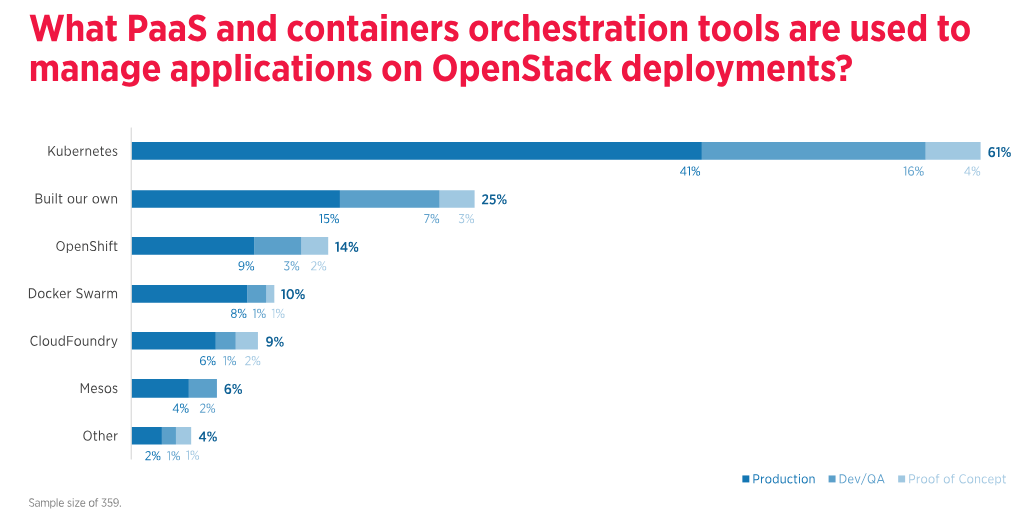
\includegraphics[width=10cm]{figures/k8s-openstack-survey.png}
	%\caption{Preferred containers orchestration tools on OpenStack, OpenStack Survey, 2018}
	\label{fig:k8s-openstack-survey}
\end{figure}
\end{frame}

\begin{frame}{Kubernetes is popular}%{{{
\begin{figure}
	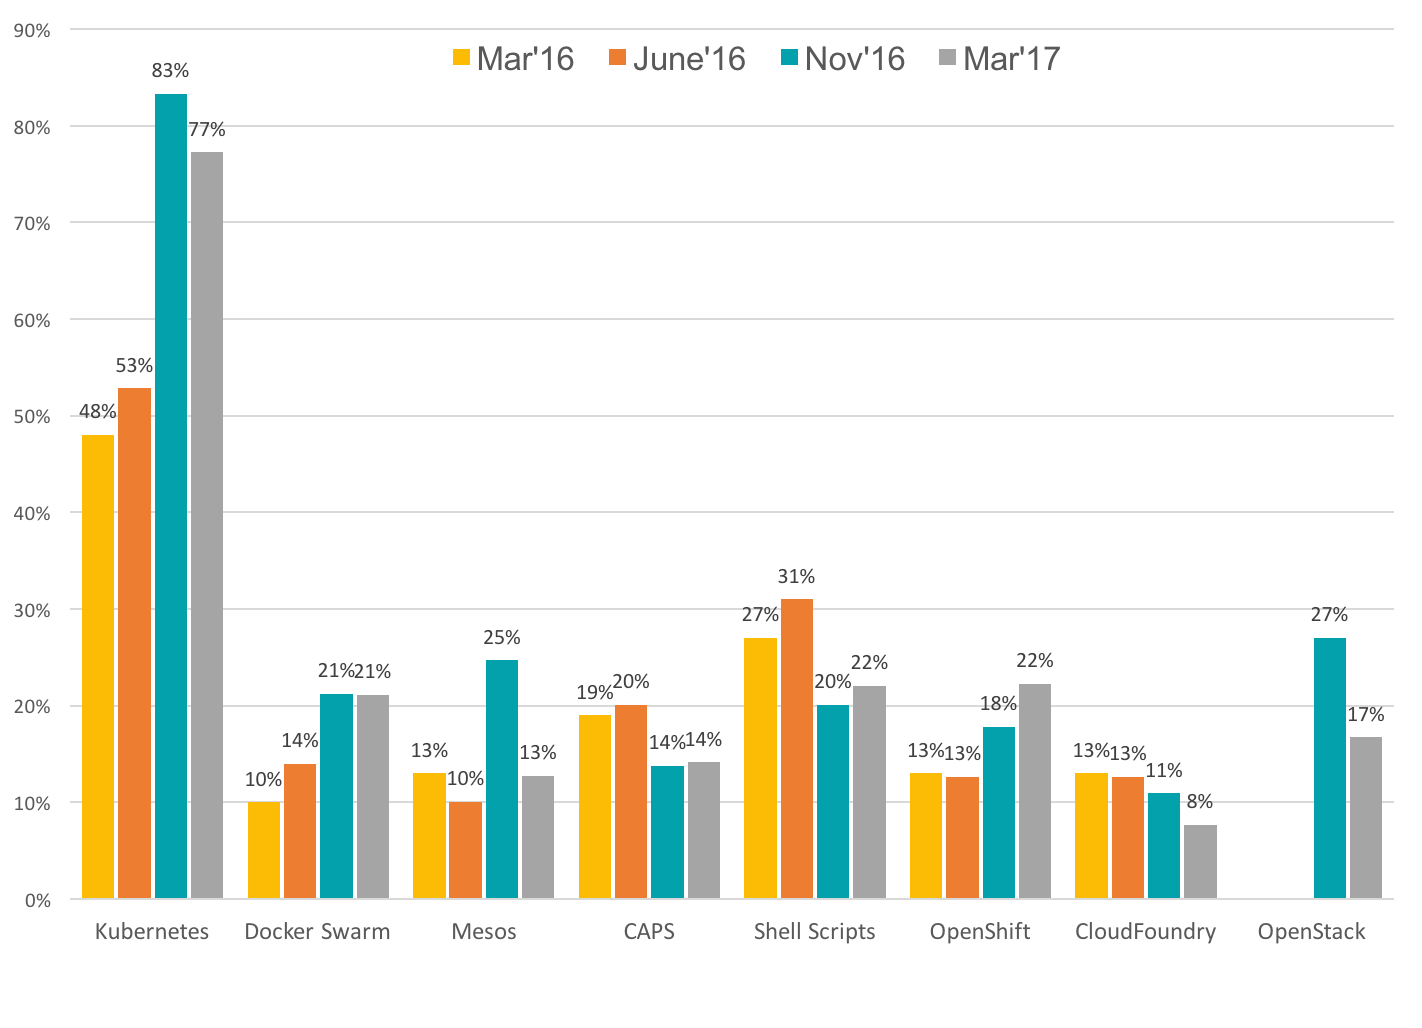
\includegraphics[width=10cm]{figures/cncf-container-orchestrators.png}
	%\caption{Preferred container management platforms, CNCF Survey, 2017}
	\label{fig:cncf-container-orchestrators}
\end{figure}
\end{frame}

% \begin{center}
% \begin{tabular}{| p{0.5\textwidth} | p{0.5\textwidth} |}
% 	\hline
% 	{\bfseries Challenges} & {\bfseries Potential solutions} \\ \hline
% 	How to deploy a microservice if it depends on many other microservices? & Use a containers' orchestrator like: Docker-compose, \textbf{Kubernetes}, Mesos, Docker Swarm \\ \hline
% 	How to ensure repetitive and fast deployments? & Use \textbf{DevOps} practices like: Infrastructure as Code, Continuous Integration, Continuous Delivery, Configuration Management Systems \\ \hline
% 	How to ensure self-healing of services (e.g. automated restarts) and diminish the number of needed for on-site engineers? &  \\ \hline
% 	How to satisfy the need for scalability? & Migrate to a public cloud which provides elastic resources; Use orchestrator like \textbf{Kubernetes} \\ \hline
% 	\hline
% \end{tabular}
% \end{center}
%}}}
% \begin{frame}{Challenges and potential solutions}%{{{
% \begin{center}
% 	\begin{tabular}{ | c | c | }
% 		\hline
% 		Challenges & Potential solutions \\ \hline
% 		How to deploy a microservice if it depends on many other microservices? & Use a containers' orchestrator like: Docker-compose, \textbf{Kubernetes}, Mesos, Docker Swarm \\ \hline
% 		How to ensure repetitive and fast deployments? & Use \textbf{DevOps} practices like: Infrastructure as Code, Continuous Integration, Continuous Delivery, Configuration Management Systems \\ \hline
% 		How to ensure self-healing of services (e.g. automated restarts) and diminish the number of needed for on-site engineers? &  \\ \hline
% 		How to satisfy the need for scalability? & Migrate to a public cloud which provides elastic resources; Use orchestrator like \textbf{Kubernetes} \\ \hline
% 	\end{tabular}
% \end{center}

% Conclusion: Kubernetes is useful.
% %}}}


\section{Problematyka}
\begin{frame}{Problematyka}%{{{
\uncover<1->{
\begin{itemize}
\item {\bfseries Bazy i hurtownie danych} -- {\bfseries {\color{red} olbrzymia
ilość liczb}}\ldots
\item \dots a ludzka percepcja jest ograniczona
\end{itemize}
}

\setbeamercovered{transparent} 
\begin{block}<2->{Wymagania użytkowników}
	{\color{blue}\bfseries Przyjazna, naturalna reprezentacja danych}
	\begin{itemize}
		\item czytelność danych i wiedzy -- {\color{blue}język naturalny} 
		\item znaczenie i kontekst -- {\color{blue} objaśnianie, podsumowywanie}
	\end{itemize}
\end{block}
\setbeamercovered{visible}
%\item {\bfseries\color{blue}Dziedzina zdecydowanie wymaga wsparcia ze strony IT}

\uncover<3->{
	\begin{center}
		\includegraphics[width=6cm]{../generator-min}
	\end{center}
} %<2->
\end{frame}

%\begin{minipage}{0.55\textwidth} \centering {\bfseries {\color{blue}Blisko połowa} pracowników ma {\color{blue}} pensję ok.  $3\,000$}\\ {\footnotesize \em zamiast}\\ {\color{red}$4807$ z $10\,000$} pracowników ma pensję {\color{red}$\geq 2000$} \end{minipage}
%}}}

\section{Zbiory rozmyte i terminy lingwistyczne}
\subsection{Reprezentacja wyrażeń nieprecyzyjnych}
\begin{frame}{Reprezentacja wyrażeń nieprecyzyjnych} %{{{

\begin{block}{Zbiór rozmyty}
\begin{equation}\label{formfs}
A = \{\langle x, \mu_A(x)\rangle\colon x \in {\cal X}\}
\end{equation}
$\mu_A\colon{\cal X}\to[0,1]$ -- funkcja przynależności [Zadeh 1965]
\end{block}

\begin{figure}
\centering
\includegraphics[width=0.6\textwidth]{../1figmftallpl.jpg}
%\caption{Reprezentacja wyrażeń ,,średni'' i ,,wysoki człowiek''}
\end{figure}

\setbeamercovered{transparent} 
\begin{itemize}
\item <2-> \textbf{Własność $\equiv$ zbiór posiadających ją obiektów}
\end{itemize}

\end{frame}
%}}}

\subsection{Spójniki, modyfikatory, wyrażenia kwantyfikowane}
\begin{frame}{Spójniki, modyfikatory, wyrażenia kwantyfikowane}%{{{
\begin{itemize}
\item ORAZ, LUB, NIE - iloczyn, suma, dopełnienie zb. rozm. 
\item BARDZO, MNIEJ WIĘCEJ, PRAWIE - modyfikatory, {\em hedges}
\begin{itemize}
\item operacje na funkcjach przynależności, np. potęgowanie
\end{itemize}
\end{itemize}

\setbeamercovered{transparent} 
\begin{block}<2->{Wyrażenia kwantyfikowane lingwistycznie}
\begin{equation} \label{eq.truthofformcanq1}
T\left(\mbox{ $Q$ $x$'ów jest $S$} \right) = \mu_Q \Big(\card(S)\Big)
\end{equation}
\begin{equation} \label{eq.truthofformcanq2}
T\left(\mbox{ $Q$ $x$'ów, które są $W$, jest $S$} \right) = \mu_Q \left(
{{\card(S \cap W)}\over{\card(W)}}  \right)
\end{equation}
\end{block}

\begin{itemize}
\item <3-> gdzie: $S, W$ -- zbiory rozmyte w $\cal X$, $Q$ -- kwantyfikator rozmyty\begin{itemize}
\item np. {\em OKOŁO POŁOWY studentów ma WYSOKĄ ŚREDNIĄ}
\end{itemize}
\end{itemize}
\end{frame}
%}}}

\subsection{Lingwistyczne podsumowania baz danych}
\begin{frame}{Lingwistyczne podsumowania baz danych}%{{{
\setbeamercovered{transparent}
		\begin{itemize}
			\item <1->{{\color{blue}Większość} pracowników ma {\color{blue}
średnią pensję}} 
\begin{itemize}
\item {\footnotesize \alert<1>{1-sza forma}, $Q^{I}$, [Yager 1982]}
\end{itemize}
\begin{equation}
T = \mu_Q\left( {{\sum\nolimits_{d_i\in{\cal D}}\mu_S(d_i)}\over|{\cal D}|}\right)
\end{equation} 
\item <2->{{\color{blue}Większość} pracowników {\bfseries\color{blue}  około 30 lat}, ma {\color{blue} średnią pensję}} 
\begin{itemize}
\item {\footnotesize \alert<2>{2-ga forma}, $Q^{II}$, [Kacprzyk, Yager, Zadrożny 2001]}
\end{itemize}
\begin{equation}
T=\mu_Q\left( {\sum\nolimits_{d_i\in{\cal D}}\mu_S(d_i)\wedge
\mu_W(d_i)}\over{\sum\nolimits_{d_i\in{\cal D}}\mu_W(d_i)}\right)
\end{equation}
\end{itemize}
gdzie ${\cal D}=\{d_1, d_2, \ldots, d_m\}$
\end{frame}
%}}}

\subsection{Generator podsumowań}
\begin{frame}{Generator podsumowań}%{{{

\setbeamercovered{transparent} 
	\begin{center}
		\includegraphics[width=0.6\textwidth]{../generator}
	\end{center}


\begin{itemize}
\item <2->{\footnotesize\bfseries
\alert<3>{Około połowy pracowników} ma \alert<4>{około 30 lat}
\alert<5>{[0.61]}. \alert<6>{Znacznie więcej niż
2000 pracowników} ma \alert<7>{wyższe wykształcenie} [0.74]. Około połowy pracowników
zarabia blisko 4000 [0.53]. Wielu pracowników \alert<8>{ma wyższe wykształcenie i
zarabia blisko 4000} [0.36]
}
\end{itemize}
\end{frame}
%}}}


\section{Zastosowania podsumowań lingwistycznych}
\subsection{Znane opracowania}
\begin{frame}{Znane opracowania}%{{{
\begin{itemize}
\setbeamercovered{transparent}
\item <1->Kacprzyk, Zadrożny 1995		-- \alert<1>{FQUERY for MS Access}
\item George, Srikanth 1996		-- \alert<2>{zastosowanie alg. genetycznych}
\item <3->Kacprzyk, Strykowski 1996	-- \alert<3>{wspomaganie marketingu}
\item <3->Ochelska 2001			-- \alert<4>{podsumowania dokumentów
medycznych}
\item <5->Kacprzyk, Zadrożny 2003		-- \alert<5>{protoformy, podsumowania interaktywne i przez internet}
\item <5->Kacprzyk, Wilbik 2007		-- \alert<6>{podsumowania szeregów
czasowych}
\item <5->wiele innych
\end{itemize}
\end{frame}
%}}}

\subsection{Prace bieżące}
\begin{frame}{Prace bieżące}%{{{
\setbeamercovered{transparent} 
 \begin{columns}
  \begin{column}{0.64\textwidth}
	\begin{itemize}
		\item <1->Podsumowania danych \alert<1>{rozmytych} poprzez {\em type-2 fuzzy sets}
	\end{itemize}
 \end{column}
 \begin{column}{0.36\textwidth}
\includegraphics[width=\textwidth]{2figfst2exc}
		\vspace{-2mm}
 \end{column}
\end{columns}

\begin{columns}
\begin{column}{0.64\textwidth}
	\begin{itemize}
		\item <2->Przyspieszone i/lub nowe algorytmy obliczania
\alert<2>{\em degrees of~truth}
	\end{itemize}
\end{column}
\begin{column}{0.36\textwidth}
   	\begin{itemize}
		\item <2>GD $O(n \log n)$
		\item <2>MVCP $O(n)$
	\end{itemize}
\end{column}
\end{columns}

\begin{columns}
\begin{column}{0.64\textwidth}
	\begin{itemize}
		\item <3->\alert<3>{Miary jakości} podsumowań
	\end{itemize}
\end{column}
\begin{column}{0.36\textwidth}
	\begin{itemize}
		\item<3> $T_1\div T_5$, $T_6\div T_{11}$, $I$, $SP(\cdot)$,
		{\em descriptors}
	\end{itemize}
\end{column}
\end{columns}

\begin{columns}
\begin{column}{0.64\textwidth}
	\begin{itemize}
		\item <4-> \alert<4>{Gramatyka i fleksja} podsumowań
	\end{itemize}
\end{column}
\begin{column}{0.36\textwidth}
	\begin{itemize}
		\item <4>Jęz. słowiańskie \vspace{1mm}\\
		\setbeamercovered{visible}
		\uncover<4>{\includegraphics[width=0.5\textwidth]{ubuntu}}
		\setbeamercovered{transparent}
	\end{itemize}
\end{column}
\end{columns}

\begin{columns}
\begin{column}{0.64\textwidth}
	\begin{itemize}
		\item <5->\alert<5->{Interfejsy} użytkownika i eksperta/-ów
	\end{itemize}
\end{column}
\begin{column}{0.36\textwidth}
	\begin{itemize}
		\item <5->Wykresy JChart, format XML
	\end{itemize}
\end{column}
\end{columns}
\end{frame}
%}}}

\subsection{Możliwości, uogólnienia}
\begin{frame}{Możliwości, uogólnienia}%{{{
\setbeamercovered{transparent}
\begin{itemize}
	\item <1->Nadal olbrzymi i \alert<1->{niewykorzystany potencjał
aplikacyjny}
 \begin{itemize}
	\item<1-> Barwise'a i Coopera teoria uogólnionej kwantyfikacji (TGQ) -- ponad
30 rodzajów kwantyfikatorów lingwistycznych (!)
\end{itemize}
\item <2-> \alert<2>{Rozszerzenia zbiorów rozmytych}
	\begin{itemize}
		\item Przedziałowe zbiory rozmyte
		\item Intuicjonistyczne zbiory rozmyte oraz {\em I-fuzzy sets}
		\item Zbiory rozmyte typu 2
		\item Zbiory przybliżone Pawlaka
	\end{itemize}
\item <3-> \alert<3->{Nowe implementacje}, w połączeniu np. z Fuzzy SQL
\end{itemize}
\end{frame}
%}}}

\subsection{Ostatnie publikacje}
\begin{frame}{Ostatnie publikacje}%{{{
\begin{itemize}
		{\scriptsize
\item {\bf Niewiadomski, A.}, {\em   On Finity, Countability, Cardinalities, And
Cylindric Extensions of~Type-2 Fuzzy Sets in Linguistic Summarization
of~Databases}, IEEE Transactions on Fuzzy Systems, 2010, (w druku).
\item {\bf Niewiadomski, A.}, Korczak, O., {\em Methods of~evaluating degrees
of~truth for~linguistic summaries of data: a~comparative~analysis}. Lecture
Notes in Artificial Intelligence, 2010, (w druku). 
\item {\bf Niewiadomski, A.}, {\em On type-2 fuzzy logic and linguistic summarization of databases}, Bulletin of the Section of Logic, Vol. 38, Nr 3/4, 2009, ss. 215--227.
\item  {\bf Niewiadomski, A.}, {\em Methods for the Linguistic
Summarization of~Data: Applications of~Fuzzy Sets and Their
Extensions}. Akademicka
Oficyna Wydawnicza EXIT, 2008. Seria IBS PAN, Badania Systemowe, tom 60. 
\item {\bf Niewiadomski, A.}, {\em A type-2 fuzzy approach to linguistic summarization of~data}, IEEE Transactions on Fuzzy Systems, Vol. 16, Nr 1, 2008, ss. 198-212. 
\item {\bf Niewiadomski, A.}, Ochelska, J., Szczepaniak, P. S., {\em Interval-
valued linguistic summaries of~databases}, Control and Cybernetics, Vol. 35, Nr
2, 2006, ss. 415-444. 

}

\end{itemize}
\end{frame}
%}}}

\end{document}

